\documentclass[master=emitm,masteroption=bc,oneside]{kulemt}
\DisemulatePackage{setspace}
\usepackage{setspace}
\usepackage{pdfpages}
\usepackage{amsmath}
\usepackage{pgf,tikz}
\usepackage{mdframed}
\usepackage{float}
\usetikzlibrary{positioning, arrows.meta, matrix, backgrounds, shapes.misc}
\usetikzlibrary{calc,arrows}
\usepackage{enumitem}

\makeatletter

%%%%%%%%%%%%%%%%%%% Begin add-int-rnd %%%%%%%%%%%%%%%
% Data Flip Flip (DFF) shape
\pgfdeclareshape{dff}{
	% The 'minimum width' and 'minimum height' keys, not the content, determine
	% the size
	\savedanchor\northeast{%
		\pgfmathsetlength\pgf@x{\pgfshapeminwidth}%
		\pgfmathsetlength\pgf@y{\pgfshapeminheight}%
		\pgf@x=0.5\pgf@x
		\pgf@y=0.5\pgf@y
	}
	% This is redundant, but makes some things easier:
	\savedanchor\southwest{%
		\pgfmathsetlength\pgf@x{\pgfshapeminwidth}%
		\pgfmathsetlength\pgf@y{\pgfshapeminheight}%
		\pgf@x=-0.5\pgf@x
		\pgf@y=-0.5\pgf@y
	}
	% Inherit from rectangle
	\inheritanchorborder[from=rectangle]
	
	% Define same anchor a normal rectangle has
	\anchor{center}{\pgfpointorigin}
	\anchor{north}{\northeast \pgf@x=0pt}
	\anchor{east}{\northeast \pgf@y=0pt}
	\anchor{south}{\southwest \pgf@x=0pt}
	\anchor{west}{\southwest \pgf@y=0pt}
	\anchor{north east}{\northeast}
	\anchor{north west}{\northeast \pgf@x=-\pgf@x}
	\anchor{south west}{\southwest}
	\anchor{south east}{\southwest \pgf@x=-\pgf@x}
	\anchor{text}{
		\pgfpointorigin
		\advance\pgf@x by -.5\wd\pgfnodeparttextbox%
		\advance\pgf@y by -.5\ht\pgfnodeparttextbox%
		\advance\pgf@y by +.5\dp\pgfnodeparttextbox%
	}
	
	% Define anchors for signal ports
	\anchor{D}{
		\pgf@process{\northeast}%
		\pgf@x=-1\pgf@x%
		\pgf@y=.5\pgf@y%
	}
	\anchor{CLK}{
		\pgf@process{\northeast}%
		\pgf@x=-1\pgf@x%
		\pgf@y=-.66666\pgf@y%
	}
	\anchor{CE}{
		\pgf@process{\northeast}%
		\pgf@x=-1\pgf@x%
		\pgf@y=-0.33333\pgf@y%
	}
	\anchor{Q}{
		\pgf@process{\northeast}%
		\pgf@y=.5\pgf@y%
	}
	\anchor{Qn}{
		\pgf@process{\northeast}%
		\pgf@y=-.5\pgf@y%
	}
	\anchor{R}{
		\pgf@process{\northeast}%
		\pgf@x=0pt%
	}
	\anchor{S}{
		\pgf@process{\northeast}%
		\pgf@x=0pt%
		\pgf@y=-\pgf@y%
	}
	% Draw the rectangle box and the port labels
	\backgroundpath{
		% Rectangle box
		\pgfpathrectanglecorners{\southwest}{\northeast}
		% Angle (>) for clock input
		\pgf@anchor@dff@CLK
		\pgf@xa=\pgf@x \pgf@ya=\pgf@y
		\pgf@xb=\pgf@x \pgf@yb=\pgf@y
		\pgf@xc=\pgf@x \pgf@yc=\pgf@y
		\pgfmathsetlength\pgf@x{1.6ex} % size depends on font size
		\advance\pgf@ya by \pgf@x
		\advance\pgf@xb by \pgf@x
		\advance\pgf@yc by -\pgf@x
		\pgfpathmoveto{\pgfpoint{\pgf@xa}{\pgf@ya}}
		%		\pgfpathlineto{\pgfpoint{\pgf@xb}{\pgf@yb}}
		%		\pgfpathlineto{\pgfpoint{\pgf@xc}{\pgf@yc}}
		\pgfclosepath
		
		% Draw port labels
		\begingroup
		\tikzset{flip flop/port labels} % Use font from this style
		\tikz@textfont
		\endgroup
	}
}

%%%%%%%%%%%%%%%%%%% End add-int-rnd %%%%%%%%%%%%%%%

% Key to add font macros to the current font
\tikzset{add font/.code={\expandafter\def\expandafter\tikz@textfont\expandafter{\tikz@textfont#1}}} 

% Define default style for this node
\tikzset{flip flop/port labels/.style={font=\sffamily\scriptsize}}
\tikzset{every dff node/.style={draw,minimum width=1.0cm,minimum 
		height=0.5cm,very thick,inner sep=1mm,outer sep=0pt,cap=round,add 
		font=\sffamily}}
%\usepackage{kulemtx}
%\headstyles{kulemtman}
%\kulemtmanToC


\setup{title={Metrics of Operating System Security Components in Virtual Environments},
  author={Oliver Jessl},
  promotor={Prof. Dr.-Ing. Clemens Martin},
  assessor={Prof. Dr.-Ing. habil. Dennis Pfisterer},
  assistant={}}
% The following \setup may be removed entirely if no filing card is wanted
\setup{filingcard,
  translatedtitle=,
  udc=621.3,
  shortabstract={Here comes a very short abstract, containing no more than 500
    words. \LaTeX\ commands can be used here. Blank lines (or the command
    \texttt{\string\pa r}) are not allowed!
    \endgraf \lipsum[2]}}
% Uncomment the next line for generating the cover page
%\setup{coverpageonly}
% Uncomment the next \setup to generate only the first pages (e.g., if you
% are a Word user.
%\setup{frontpagesonly}

\setlrmarginsandblock{3cm}{3cm}{*}
\setulmarginsandblock{3cm}{3cm}{*}
\checkandfixthelayout

% Choose the main text font (e.g., Latin Modern)
\setup{font=times}

% If you want to include other LaTeX packages, do it here. 

% Finally the hyperref package is used for pdf files.
% This can be commented out for printed versions.
\usepackage[pdfusetitle,colorlinks,plainpages=false]{hyperref}

%%%%%%%
% The lipsum package is used to generate random text.
% You never need this in a real master's thesis text!
\IfFileExists{lipsum.sty}%
 {\usepackage{lipsum}\setlipsumdefault{11-13}}%
 {\newcommand{\lipsum}[1][11-13]{\par And some text: lipsum ##1.\par}}
%%%%%%%



%\onehalfspacing
\onehalfspacing

%\includeonly{chap-n}
\begin{document}



\begin{preface}
  I would like to thank everybody who kept me busy the last year,
  especially my promoter and my assistants. I would also like to thank the
  jury for reading the text. My sincere gratitude also goes to my wive and
  the rest of my family.
\end{preface}



\tableofcontents*

\begin{abstract}
  The \texttt{abstract} environment contains a more extensive overview of
  the work. But it should be limited to one page.

  \lipsum[1]
\end{abstract}

% A list of figures and tables is optional
%\listoffigures
%\listoftables
% If you only have a few figures and tables you can use the following instead
\listoffiguresandtables
% The list of symbols is also optional.
% This list must be created manually, e.g., as follows:
\chapter{List of Abbreviations and Symbols}
\section*{Abbreviations}
\begin{flushleft}
  \renewcommand{\arraystretch}{1.1}
  \begin{tabularx}{\textwidth}{@{}p{12mm}X@{}}
    ASLR  & Address Space Randomization Layout \\  	
    GRI   & Get Random Int (Random Number Generator)\\
	GRL	  & Get Random Long (Random Number Generator)\\
    NIST  & National Institute of Standards and Technology \\
    PRNG  & Pseudo Random Number Generator \\    
    TRNG  & True Random Number Generator \\        
    VM	  & Virtual Machine \\
  \end{tabularx}
\end{flushleft}
\section*{Symbols}
\begin{flushleft}
  \renewcommand{\arraystretch}{1.1}
  \begin{tabularx}{\textwidth}{@{}p{12mm}X@{}}
    42    & ``The Answer to the Ultimate Question of Life, the Universe,
            and Everything'' according to \cite{h2g2} \\
    $c$   & Speed of light \\
    $E$   & Energy \\
    $m$   & Mass \\
    $\pi$ & The number pi \\
  \end{tabularx}
\end{flushleft}


% Now comes the main text
\mainmatter

\chapter{Introduction}
\label{cha:intro}
\section{Motivation}
Operating systems implement a variety of security components which depend significantly on the entropy of random numbers. In general, those random numbers can be provided by operating system internal or external providers, so called Random Number Generators (RNG). Typical external providers are hardware devices, able to deviate random numbers from radioactive decay, atmospheric or thermal noise, photoelectric effects etc. Since those numbers are assumed to provide a high level of entropy i.e. random numbers of high quality, they are also referred as True Random Number Generators (TRNG). Contrary, RNGs implemented as part of an operating system, the lack of comparable stochastic processes and hence are labeled as Pseudo Random Number Generator (PRNG). To compensate this lack, PRGN implementations need to fall back on alternative sources, able to provide information with a certain degree of entropy. Common approaches of operating systems usually adopt information from external sources, f.e. user input like keyboard events or mouse coordinates. Beside further external input like network traffic, system internal individual information like serial numbers of hardware devices, MAC addresses or the occurrence of hardware interrupts is used to gain an entropy pool of pseudo random numbers. Consequently, the process of generating random numbers by an operating system PRNG is influenced by the way the system interacts with its environment i.e. how it is set up. This aspect should be considered when applying server operating systems as virtual machines i.e. in virtual environments. \\~\\
Virtualization of operating systems has increased continuously over the recent years and layed the foundations for new resource management concepts and business models like f.e. cloud hosting. Regarding server virtualization, many organizations exceed rates of 75\% \cite{gartnervmmarket}. By executing an operating system as a virtual machine, improvements in several areas, like scalability and more efficient utilization of hardware resources, backup \& disaster recovery strategy, accelerated provision of new system instances etc. can be achieved. Depending on the applied technology, such virtual machines can be setup up on basis of operating system setup images which are targeted for installation directly on hardware, without any further modification required. In other words, the virtual machine monitor or hypervisor enables the execution of regular commercial or open source operating systems in a virtual environment. However, while there are many reasons to utilize virtual machines, most of the standard security practices of operating systems are based on assumptions that hold true for physical machines, but don't translate immediately into the domain of virtualized machines \cite{kerrigan2012study}. A virtual hosted Linux server f.e. will never receive a user triggered event during the boot process, which is a critical period within the initialization of the internal Linux PRNG. Further, new virtual machine instances are usually provided by cloning a master image, instead of running an installation setup, leading to a higher degree of homogeneity among virtual machine instances. While provisioning time and maintenance benefit from this practice, it may be regarded critical. If this approach f.e. is applied as the standard process of a cloud hosting provider, it`s customers may be delivered a vulnerable system from the outset, since one customer might gain insights regarding another customers system, just by analyzing his own. These insights can be used to exploit VM reset vulnerabilities which take advantage of the reuse of  operating system snapshots, so called snapshot replay. Thomas Ristenpart et. al. describe this type of attack and apply it on TSL implementations with disastrous results. Relevant reasons they identified are the exposure of randomness, as well as the inability to find sufficient entropy in virtual systems environments \cite{ristenpart2010good, ristenpart2009hey}. \\~\\
According to a study of Gartner from 2016, the market for x86 server virtualization infrastructure software is partitioned among few competitors, led by VMWare, Microsoft, Oracle and Red Hat. While VMWare and Microsoft offer proprietary solutions, Oracle and Red Hat adopted the open-source Xen-hypervisor technology. For cloud infrastructures, the Xen-hypervisor remains the most widely used architecture for public infrastructure as a service (IaaS) cloud provider. This fact is predominantly attributable to Amazon's utilization of the Xen-hypervisor for its cloud solutions "Amazon Web Services" \cite{bittman2016magic}. Similarly, the market of common server operating systems can be divided into proprietary and open-source solutions. While Microsoft dominates the fraction of proprietary systems with its Windows Server series, Linux based systems have a total share of \~37\%. Within this share, \~39\% of servers dedicated to host websites etc. are running an Ubuntu Distribution \cite{statsharelinux} . \\~\\
Summarized, recent studies have revealed that virtualization of Linux based servers is widespread, while the execution of those systems as virtual machine may bring up critical vulnerabilities. Based on these considerations the objective of this thesis is an analysis of the generation of random numbers by a Linux 4.X.X.X kernel's internal PRNG in a Xen-hypervisor environment. To this date, several research contributions have been published in this field. Those may be divided by their scope regarding the Linux PRNG responsibilities, attack vectors and, if analyzing the entropy pools state, the approach of assessing randomness. While some papers address the PRNG output for the entire time of a system's uptime, the focus of this research will be a system's startup i.e. boot phase. This period is meant to be of certain interest for several reasons: The initialization of the Linux PRMG is beginning as one of the first activities conducted when a (virtual) machine starts to bring up the systems kernel, as it is eager to use as many noise sources as possible to build up various entropy pools. Further, during this initialization process, some buffers are assigned with values which are valid and reused over the entire uptime of the system. Poorly developed values for these buffers are assumed to weaken a number of security components and hence are of particular interest. Finally, a part of the boot process is the startup of various daemon processes, which usually remain in execution over the entire system uptime. Beside daemons required by the system, this may also be applications like web-, ftp-, ssh-, proxy-servers which may be reachable via the internet and thus potentially vulnerabilities should be classified as critical.
To obtain a comprehensive data record for evaluation, a Linux 4.X.X.X kernel has been enhanced by a tracking feature, able to record information at points of interest, without producing any noise itself. The feature is not just able to track the values returned to applications requesting random values, but also to breakdown how those have been generated over several stages until their origin in terms of noise. This kernel is brought up within an Ubuntu Server 16.04 system, hosted as a guest on Xen hypervisor 4.XX. The Linux PRNG has an internal rating system describing an entropy pools quality in "bits of entropy". Some research contributions (f.e. \cite{lacharme2012linux})refer to this system when assessing random number quality. To conduct an independent and fine grained analysis, for this thesis a Statistical Test Suite, published by the NIST has been applied \cite{paul2016nist}. Various operating systems security concepts rely on solid random numbers. Hence, besides the processing of noise to random numbers, also the consequences of weak random numbers have been analyzed on the effectiveness of two fundamental operating system security technologies: Stack Guards/Stack Canaries and Address Space Randomization Layout (ASLR).
The following sections will deliver the required background knowledge regarding virtualization via the Xen-hyperisor, the architecture and generation of the Linux Pseudo Random Number Generator, the concepts of stack canaries and ASLR and Statistical Random Number Validation. 



\section{Related Reserach}

Xen

----------------

ASLR

----------------

XEN/PRNG

If the correlation between the jiffies counter J and the cycle counter CC is known (they are based on the same underlying clock), then the only unknown to an attacker is CC at the time each output is generated. \cite{everspaugh2014not} VMWare beginnt mit CC=0 => katastrophal \cite{everspaugh2014not} Seite 8. Dort ansetzten, ist es bei Xen ebenso?

----------------











% Virtualization in these terms means, that an operating system is not directly installed on a hardware host. Instead on the host machine an application is installed beeing able administer systems resources and assign those to several operating systems which may be run on host simultaneously.  

   





%%% Local Variables: 
%%% mode: latex
%%% TeX-master: "thesis"
%%% End: 

\chapter{The First Chapter}
\label{cha:1}
The following section will deliver the relevant information regarding memory management an ASLR.

% EVP (Enhanced Virus Protection) – available on
all 64-bit AMD CPUs (starting in 2003)
\cite{guide2017amd64}

% XD Bit (Execute Disable Bit) – available with
Pentium 4 "Prescott" core (starting in 2004)1
\cite{guide2017intel}
If the execute-disable bit of a memory page is set, that page can be used only as data. An attempt to execute code
from a memory page with the execute-disable bit set causes a page-fault exception.

\section{Memory Management}
Modern Operation System implement an abstraction layer.

Load elf: sections -> segments.
-------------------------------------------
Virtual Address space (linearer Adressraum)
--------------------------------------------
Linear Address Space
From a user perspective, the address space is a at linear address space but pre-
dictably, the kernel's perspective is very different. The address space is split into
two parts, the userspace part which potentially changes with each full context switch
and the kernel address space which remains constant. The location of the split is
determined by the value of PAGE\_OFFSET which is at 0xC0000000 on the x86. This
means that 3GiB is available for the process to use while the remaining 1GiB is
always mapped by the kernel. The linear virtual address space as the kernel sees it
is illustrated in Figure 4.1.
\cite{gorman2004linuxvmmgr}


Up Down Kernel/User space
--------------------------












\cite{cowan2000buffer}
\cite{marco2014effectiveness}
\cite{kerrigan2012study}
\cite{guide2017intel}
\cite{wojtczuk2011following}
\cite{alt2015entropy}
\cite{thompsonrandomness}
\cite{celesti2010improving}
\cite{mueller@bsi1}
\cite{mueller@bsi2}
\cite{marco2013preventing}


%\section{The First Topic of the Chapter}
%First comes the introduction to this topic.
%
%\lipsum[55]
%
%\subsection{An item}
%Please don't abuse enumerations: short enumerations shouldn't use
%``\verb|itemize|'' or ``\texttt{enumerate}'' environments.
%So \emph{never write}: 
%\begin{quote}
%  The Eiffel tower has three floors:
%  \begin{itemize}
%  \item the first one;
%  \item the second one;
%  \item the third one.
%  \end{itemize}
%\end{quote}
%But write:
%\begin{quote}
%  The Eiffel tower has three floors: the first one, the second one, and the
%  third one.
%\end{quote}
%
%\section{A Second Topic}
%\lipsum[64]
%
%\subsection{Another item}
%\lipsum[56-57]
%
%\section{Conclusion}
%The final section of the chapter gives an overview of the important results
%of this chapter. This implies that the introductory chapter and the
%concluding chapter don't need a conclusion.
%
%\lipsum[66]

%%% Local Variables: 
%%% mode: latex
%%% TeX-master: "thesis"
%%% End: 

\chapter{The Next Chapter}
\label{cha:2}

\section{Operating System Virtualization with the Xen-Hypervisor}

Virtualization of operating systems has increased continuously over the recent years and layed the foundations for new resource management concepts and business models like f.e. cloud hosting. Regarding server virtualization, many organizations exceed rates of 75\% \cite{gartnervmmarket}. By executing an operating system as a virtual machine (VM), improvements in several areas can be achieved. As instances of even different operating systems can be run parallel on the same host machine, system capacity in terms of processing power, volatile and persistent memory can be utilized more efficient. A VM can even be assigned resources dynamically at runtime, without the need of a restart. Further, backup \& recovery strategies can be simplified, as a VM's physical presentation at any certain state can be preserved in files. This even enables to move a running VM from one to another server in the same resource pool with virtually no service interruption \cite{migratevms}. Also the process of providing a new VM instance can be slimmed down drastically. Instead of being required to execute an operating system setup for a particular hardware composition, a once created VM master image can be cloned and configured. Depending on the applied technology, VMs can be setup up on basis of operating system setup images which are targeted for installation directly on hardware, without any further modification required. In other words, the virtual machine monitor or hypervisor enables the execution of regular proprietary or open source operating systems in a virtual environment. \\
According to a study of Gartner from 2016, the market for x86 server virtualization infrastructure software is partitioned among few competitors, led by VMWare, Microsoft, Oracle and Red Hat. While VMWare and Microsoft offer proprietary solutions, Oracle and Red Hat adopted the open-source Xen-hypervisor technology. For cloud infrastructures, the Xen-Hypervisor remains the most widely used architecture for public infrastructure as a service (IaaS) cloud provider. This fact is predominantly attributable to Amazon's utilization of the Xen-Hypervisor for its cloud solutions "Amazon Web Services" \cite{bittman2016magic}.
\\~\\
Hier muss noch ein Uebergang hin
\\


- Open Source
- Amazon
- Verbreitung 
- HVM / PVM
- Architektur

------------------------------------
\cite{everspaugh2014not}
Second,aVM  can be repeatedly executed froma ?xed image which is the default for amazon
Dort auch: infos zu regualr boot/snapshot/masterimage
------------------------------------



However, while there are many reasons to utilize virtual machines, most of the standard security practices of operating systems are based on assumptions that hold true for physical machines, but don't translate immediately into the domain of virtualized machines \cite{kerrigan2012study}. A virtual hosted Linux server f.e. will never receive a user triggered event during the boot process, which is a critical period within the initialization of the internal Linux PRNG. Further, new virtual machine instances are usually provided by cloning a master image, instead of running an installation setup, leading to a higher degree of homogeneity among virtual machine instances. While provisioning time and maintenance benefit from this practice, it may be regarded critical. If this approach f.e. is applied as the standard process of a cloud hosting provider, it`s customers may be delivered a vulnerable system from the outset, since one customer might gain insights regarding another customers system, just by analyzing his own. These insights can be used to exploit VM reset vulnerabilities which take advantage of the reuse of  operating system snapshots, so called snapshot replay. Thomas Ristenpart et. al. describe this type of attack and apply it on TSL implementations with disastrous results. Relevant reasons they identified are the exposure of randomness, as well as the inability to find sufficient entropy in virtual systems environments \cite{ristenpart2010good, ristenpart2009hey}. \\~\\
According to a study of Gartner from 2016, the market for x86 server virtualization infrastructure software is partitioned among few competitors, led by VMWare, Microsoft, Oracle and Red Hat. While VMWare and Microsoft offer proprietary solutions, Oracle and Red Hat adopted the open-source Xen-hypervisor technology. For cloud infrastructures, the Xen-hypervisor remains the most widely used architecture for public infrastructure as a service (IaaS) cloud provider. This fact is predominantly attributable to Amazon's utilization of the Xen-hypervisor for its cloud solutions "Amazon Web Services" \cite{bittman2016magic}. 

Similarly, the market of common server operating systems can be divided into proprietary and open-source solutions. While Microsoft dominates the fraction of proprietary systems with its Windows Server series, Linux based systems have a total share of \~37\%. Within this share, \~39\% of servers dedicated to host websites etc. are running an Ubuntu Distribution \cite{statsharelinux} . \\~\\


\section{Random Number Generation in Linux x64 Kernel 4.4}

\subsection{General}

Random numbers are required by a variety of security related applications. An obvious purpose is encryption or signing of data, like f.e. disk encryption, Transport Socket Layer (TLS) or digital signatures of emails. In this case random numbers are used to generate cryptographically secure keys. Concepts like Stack Canaries (aka. Stack Guards) or Address Space Layout Randomization (ASLR) rely purely on the nondeterministic character of random numbers, applying them to make certain types of attacks on vulnerable applications much more difficult. Overall, the effectiveness of such applications depends significantly on the quality i.e. unpredictably of random numbers, provided by an operating system. \\
In the following a comprehensive introduction to the Linux Random Number Generator (LRNG) with focus on analyzed concepts and components of this thesis will be given. It refers to Linux kernel v.4.4, which is currently used in several major Long Term Support distributions like Ubuntu Server 16.04 LTS. If facts are valid for Intel x86/x64 platforms only, those will be noted as such.\\
In general, many modern CPU-architectures implement an on-chip True Random Number Generator \cite{guide2017intel}. Starting with 'IvyBridge' architecture, Intel provides two instructions accessing directly those entropy sources. The \textsf{RDRAND} instruction returns random numbers that are supplied by a cryptographically secure, deterministic random bit generator (DRBG). The DRBG is designed to meet the NIST SP 800-90A standard. If an application or operating system design insists on applying in it's own Pseudo Random Number Generator (PRNG) it may apply the \textsf{RDSEED} instruction which is compliant to NIST SP 800-90B \& C standard \cite{guide2017intel}.
Availability of these TRNGs does not automatically imply their application. If a kernel is started 
with paramter \textsf{nordrand} (on x86/x64 architectures), the \textsf{RDRAND} instruction will have no effect. Further, if an operating system is run as a virtual machine, those instructions can by trapped by the hypervisor instead of being passed to the CPU \cite{mueller@bsi2}. Thus the analysis in this thesis does not take on-chip entropy pools into account, but refers to the pure Linux Pseudo Random Number Generator).

\subsection{Linux Pseudo Random Number Generator Architecture}
The Linux Pseudo Random Number Generator's (PRNG) responsibility is to provide random numbers to requesting consumers. To ensure a certain quality of randomness the implementations activity may be divided into four major tasks:   

\centering
\begin{itemize}
	\item Capturing and processing input data which is finally stored in entropy pools
	\item Assessing the level of entropy in each pool
	\item Diverting incoming entropy 
\end{itemize}


generates random numbers based on occurring hardware events. Those events 


\begin{comment}
Jegliche Nutzung der RDRAND-Instruktion kann verhindert werden, wenn der Kern mit der
Kommandozeilenoption ?nordrand? gestartet wird.
Es ist zu beachten, dass RDRAND von einem Hypervisor im Sinne eines VM-Exits abgefangen
und ver�ndert beziehungsweise nicht an die CPU weitergegeben werden kann.

\end{comment}


implementation

Intel IvyBridge x86 



Intro:
valid kernel for x64  4.4. (16.04 LTS)
MISP 

 

arch:
Intel IvyBridge x86-Prozessorgeneration
TRNG
 \cite guide2017intel
RDRAND returns random numbers that are supplied by a cryptographically secure, deterministic random bit generator DRBG. The DRBG is designed to meet the NIST SP 800-90A standard.
RDSEED
Non-deterministic random bit generator
NIST SP 800-90B \& C
\cite{guide2017intel}


Diff: kernel/Userspace request

\begin{comment}
Aktuelle Arbeiten zeigen, dass gerade im Bereich von Headless-Systemen, die beim
ersten Systemstart Zufallszahlen f�r die Erzeugung von Schl�sseln ben�tigen, zu
wenig Entropie vorhanden ist. Auch wenn von den Interrupts nicht viel Entropie zu
erwarten ist, sollte die Verwendung der Interrupt-Ereignisse dieses Problem etwas
abmildern.
\cite{mueller@bsi2}
\end{comment}


\begin{figure}[H]
%\centering


%\makeatother


	
	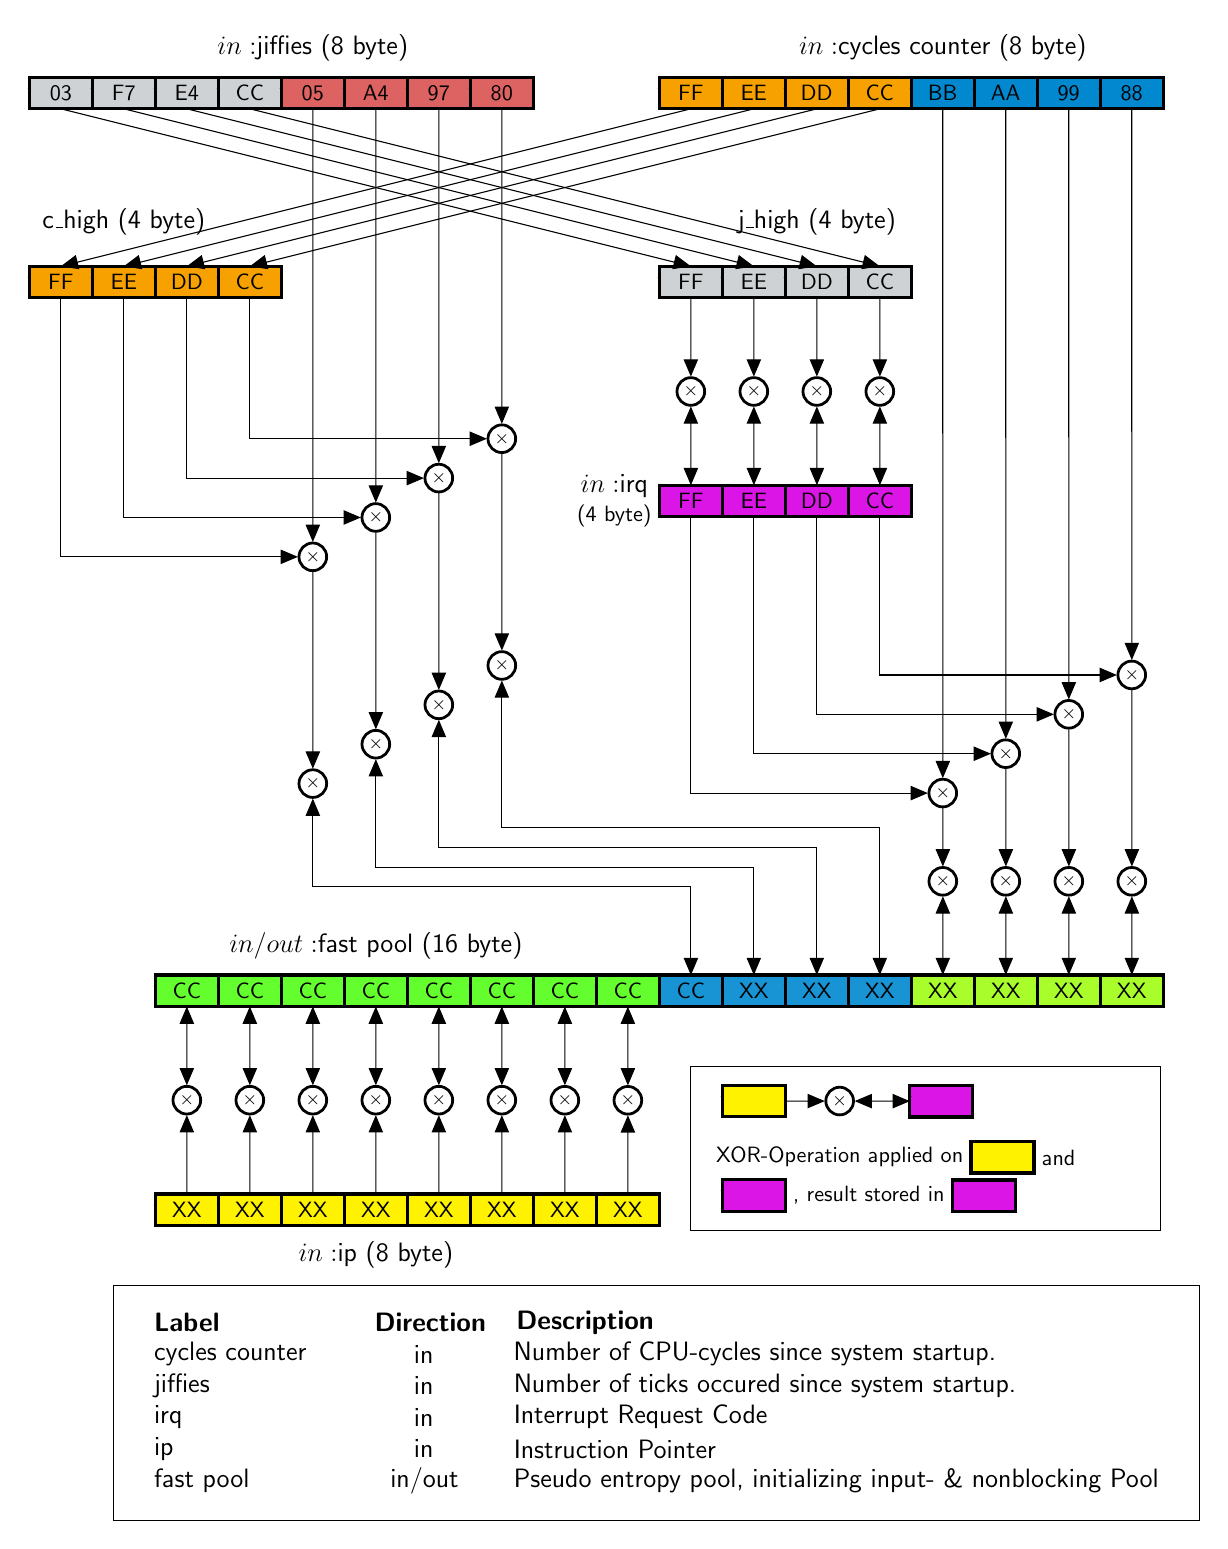
\begin{tikzpicture}[scale=0.8, every node/.style={scale=0.8},font=\sffamily,>=triangle 45]
	\tikzstyle{sum} = [draw, shape=circle, node distance=1.5cm, line width=1pt, minimum width=1.25em]	
	%\Huge
	\def\N{7}  % Number of Flip-Flops minus one
	\def\BW{1.8} % Byte Width

	% colors
	\definecolor{cjh}{HTML}{CFD2D4}
	\definecolor{cjl}{HTML}{DD6262}
	\definecolor{cch}{HTML}{F7A100}
	\definecolor{ccl}{HTML}{0288CF}
	\definecolor{cep32}{HTML}{64FE2E}
	\definecolor{cep1}{HTML}{1893D4}
	\definecolor{cep0}{HTML}{A9FD2A}
	\definecolor{cirq}{HTML}{DB15E5}
	\definecolor{cip}{HTML}{FFF200}

	% jiffies
	\node [shape=dff,fill=cjh] (jiff7) at ($ 1.0*(0,0) $) {03};
	\node [shape=dff,fill=cjh] (jiff6) at ($ 1.0*(1,0) $) {F7};
	\node [shape=dff,fill=cjh] (jiff5) at ($ 1.0*(2,0) $) {E4};
	\node [shape=dff,fill=cjh] (jiff4) at ($ 1.0*(3,0) $) {CC};			
	\node [shape=dff,fill=cjl] (jiff3) at ($ 1.0*(4,0) $) {05};
	\node [shape=dff,fill=cjl] (jiff2) at ($ 1.0*(5,0) $) {A4};
	\node [shape=dff,fill=cjl] (jiff1) at ($ 1.0*(6,0) $) {97};
	\node [shape=dff,fill=cjl] (jiff0) at ($ 1.0*(7,0) $) {80};	
	\node[above=1mm of jiff3] (ljiffies) {\large $in:$jiffies (8 byte)};		

	% jiffies low XOR c_high - XOR nodes
	\node [sum, below=4.0cm of jiff0, draw] (xjlch0) {};
	\node [sum, below=4.5cm of jiff1, draw] (xjlch1) {};	
	\node [sum, below=5.0cm of jiff2, draw] (xjlch2) {};
	\node [sum, below=5.5cm of jiff3, draw] (xjlch3) {};	
	\node [rotate=45] at (xjlch0) (plus) {{\footnotesize$+$}};
	\node [rotate=45] at (xjlch1) (plus) {{\footnotesize$+$}};	
	\node [rotate=45] at (xjlch2) (plus) {{\footnotesize$+$}};
	\node [rotate=45] at (xjlch3) (plus) {{\footnotesize$+$}};
		
	% cycles
	\node [shape=dff,fill=cch] (cycl7) at ($ 1.0*(10,0) $) {FF};
	\node [shape=dff,fill=cch] (cycl6) at ($ 1.0*(11,0) $) {EE};
	\node [shape=dff,fill=cch] (cycl5) at ($ 1.0*(12,0) $) {DD};
	\node [shape=dff,fill=cch] (cycl4) at ($ 1.0*(13,0) $) {CC};			
	\node [shape=dff,fill=ccl] (cycl3) at ($ 1.0*(14,0) $) {BB};
	\node [shape=dff,fill=ccl] (cycl2) at ($ 1.0*(15,0) $) {AA};
	\node [shape=dff,fill=ccl] (cycl1) at ($ 1.0*(16,0) $) {99};
	\node [shape=dff,fill=ccl] (cycl0) at ($ 1.0*(17,0) $) {88};
	\node[above=1mm of cycl3] (lcycles) {\large $in:$cycles counter (8 byte)};	

	%c_high
	\node [shape=dff,fill=cch, below=2cm of jiff7, draw] (chigh3) {FF};
	\node [shape=dff,fill=cch, below=2cm of jiff6, draw] (chigh2) {EE};
	\node [shape=dff,fill=cch, below=2cm of jiff5, draw] (chigh1) {DD};
	\node [shape=dff,fill=cch, below=2cm of jiff4, draw] (chigh0) {CC};
	\node[above=3mm of chigh2] (lchigh) {\large c\_high (4 byte)};			

	%j_high
	\node [shape=dff,fill=cjh, below=2cm of cycl7, draw] (jiffh3) {FF};
	\node [shape=dff,fill=cjh, below=2cm of cycl6, draw] (jiffh2) {EE};
	\node [shape=dff,fill=cjh, below=2cm of cycl5, draw] (jiffh1) {DD};
	\node [shape=dff,fill=cjh, below=2cm of cycl4, draw] (jiffh0) {CC};
	\node[above=3mm of jiffh1] (ljhigh) {\large j\_high (4 byte)};			

	% jiffies high XOR irq - XOR nodes
	\node [sum, below=1.0cm of jiffh3, draw] (xjhi3) {};	
	\node [rotate=45] at (xjhi3) (plus) {{\footnotesize$+$}};
	\node [sum, below=1.0cm of jiffh2, draw] (xjhi2) {};	
	\node [rotate=45] at (xjhi2) (plus) {{\footnotesize$+$}};
	\node [sum, below=1.0cm of jiffh1, draw] (xjhi1) {};	
	\node [rotate=45] at (xjhi1) (plus) {{\footnotesize$+$}};
	\node [sum, below=1.0cm of jiffh0, draw] (xjhi0) {};	
	\node [rotate=45] at (xjhi0) (plus) {{\footnotesize$+$}};
			
	%irq
	\node [shape=dff,fill=cirq, below=1cm of xjhi3, draw] (irq3) {FF};
	\node [shape=dff,fill=cirq, below=1cm of xjhi2, draw] (irq2) {EE};
	\node [shape=dff,fill=cirq, below=1cm of xjhi1, draw] (irq1) {DD};
	\node [shape=dff,fill=cirq, below=1cm of xjhi0, draw] (irq0) {CC};
	\node[left=0mm of irq3] (lirq) {\shortstack{\large $in:$irq\\(4 byte)}};	
	
	% cycles low XOR irq - XOR nodes
	\node [sum, below=8.5cm of cycl3, draw] (xcli3) {};
	\node [sum, below=8.0cm of cycl2, draw] (xcli2) {};	
	\node [sum, below=7.5cm of cycl1, draw] (xcli1) {};		
	\node [sum, below=7.0cm of cycl0, draw] (xcli0) {};			
	\node [rotate=45] at (xcli3) (plus) {{\footnotesize$+$}};
	\node [rotate=45] at (xcli2) (plus) {{\footnotesize$+$}};	
	\node [rotate=45] at (xcli1) (plus) {{\footnotesize$+$}};
	\node [rotate=45] at (xcli0) (plus) {{\footnotesize$+$}};	
	
	% entropy pool	
	\node [shape=dff,fill=cep32, below=11cm of jiff5, draw] (entp15) {CC};		
	\node [shape=dff,fill=cep32, below=11cm of jiff4, draw] (entp14) {CC};
	\node [shape=dff,fill=cep32, below=11cm of jiff3, draw] (entp13) {CC};
	\node [shape=dff,fill=cep32, below=11cm of jiff2, draw] (entp12) {CC};
	\node [shape=dff,fill=cep32, below=11cm of jiff1, draw] (entp11) {CC};
	\node [shape=dff,fill=cep32, below=11cm of jiff0, draw] (entp10) {CC};
	\node [shape=dff,fill=cep32, right=0cm of entp10, draw] (entp9) {CC};	
	\node [shape=dff,fill=cep32, right=0cm of entp9, draw] (entp8) {CC};
	\node [shape=dff,fill=cep1, right=0cm of entp8, draw] (entp7) {CC};
	\node [shape=dff,fill=cep1, below=11cm of cycl6, draw] (entp6) {XX};	
	\node [shape=dff,fill=cep1, below=11cm of cycl5, draw] (entp5) {XX};	
	\node [shape=dff,fill=cep1, below=11cm of cycl4, draw] (entp4) {XX};	
	\node [shape=dff,fill=cep0, below=11cm of cycl3, draw] (entp3) {XX};	
	\node [shape=dff,fill=cep0, below=11cm of cycl2, draw] (entp2) {XX};	
	\node [shape=dff,fill=cep0, below=11cm of cycl1, draw] (entp1) {XX};	
	\node [shape=dff,fill=cep0, below=11cm of cycl0, draw] (entp0) {XX};	
	\node[above=1mm of entp12] (lentp) {\large $in/out:$fast pool (16 byte)};	

	%% XOR entp
	% ch / jl 
	\node [sum, below=2.5cm of xjlch3, draw] (xentp7) {};	
	\node [rotate=45] at (xentp7) (plus) {{\footnotesize$+$}};
	\node [sum, below=2.5cm of xjlch2, draw] (xentp6) {};	
	\node [rotate=45] at (xentp6) (plus) {{\footnotesize$+$}};
	\node [sum, below=2.5cm of xjlch1, draw] (xentp5) {};	
	\node [rotate=45] at (xentp5) (plus) {{\footnotesize$+$}};
	\node [sum, below=2.5cm of xjlch0, draw] (xentp4) {};	
	\node [rotate=45] at (xentp4) (plus) {{\footnotesize$+$}};									
	% irq/cycl 
	\node [sum, above=1.0cm of entp3, draw] (xentp3) {};	
	\node [rotate=45] at (xentp3) (plus) {{\footnotesize$+$}};
	\node [sum, above=1.0cm of entp2, draw] (xentp2) {};	
	\node [rotate=45] at (xentp2) (plus) {{\footnotesize$+$}};
	\node [sum, above=1.0cm of entp1, draw] (xentp1) {};	
	\node [rotate=45] at (xentp1) (plus) {{\footnotesize$+$}};
	\node [sum, above=1.0cm of entp0, draw] (xentp0) {};	
	\node [rotate=45] at (xentp0) (plus) {{\footnotesize$+$}};		
	% ip
	\node [sum, below=1.0cm of entp15, draw] (xentp15) {};	
	\node [rotate=45] at (xentp15) (plus) {{\footnotesize$+$}};
	\node [sum, below=1.0cm of entp14, draw] (xentp14) {};	
	\node [rotate=45] at (xentp14) (plus) {{\footnotesize$+$}};
	\node [sum, below=1.0cm of entp13, draw] (xentp13) {};	
	\node [rotate=45] at (xentp13) (plus) {{\footnotesize$+$}};
	\node [sum, below=1.0cm of entp12, draw] (xentp12) {};	
	\node [rotate=45] at (xentp12) (plus) {{\footnotesize$+$}};		
	\node [sum, below=1.0cm of entp11, draw] (xentp11) {};	
	\node [rotate=45] at (xentp11) (plus) {{\footnotesize$+$}};
	\node [sum, below=1.0cm of entp10, draw] (xentp10) {};	
	\node [rotate=45] at (xentp10) (plus) {{\footnotesize$+$}};
	\node [sum, below=1.0cm of entp9, draw] (xentp9) {};	
	\node [rotate=45] at (xentp9) (plus) {{\footnotesize$+$}};
	\node [sum, below=1.0cm of entp8, draw] (xentp8) {};	
	\node [rotate=45] at (xentp8) (plus) {{\footnotesize$+$}};	

	\node [shape=dff,fill=cip, below=1cm of xentp15, draw] (ip7) {XX};	
	\node [shape=dff,fill=cip, below=1cm of xentp14, draw] (ip6) {XX};
	\node [shape=dff,fill=cip, below=1cm of xentp13, draw] (ip5) {XX};
	\node [shape=dff,fill=cip, below=1cm of xentp12, draw] (ip4) {XX};
	\node [shape=dff,fill=cip, below=1cm of xentp11, draw] (ip3) {XX};
	\node [shape=dff,fill=cip, below=1cm of xentp10, draw] (ip2) {XX};
	\node [shape=dff,fill=cip, below=1cm of xentp9, draw] (ip1) {XX};
	\node [shape=dff,fill=cip, below=1cm of xentp8, draw] (ip0) {XX};
	\node[below=1mm of ip4] (lip) {\large $in:$ip (8 byte)};	

	%%%%%% LINES >>
	
	% jiffies  -> c_low - lines
	\draw [->] (jiff3.south) -- (xjlch3.north);
	\draw [->] (jiff2.south) -- (xjlch2.north);	
	\draw [->] (jiff1.south) -- (xjlch1.north);		
	\draw [->] (jiff0.south) -- (xjlch0.north);		

	% c_high -> xjlch
	\draw [->] (chigh3.south)|- (xjlch3.west);
	\draw [->] (chigh2.south)|- (xjlch2.west);
	\draw [->] (chigh1.south)|- (xjlch1.west);
	\draw [->] (chigh0.south)|- (xjlch0.west);			

	% jiffies high -> j_high
	\draw [->] (jiff7.south) -- (jiffh3.north);
	\draw [->] (jiff6.south) -- (jiffh2.north);	
	\draw [->] (jiff5.south) -- (jiffh1.north);		
	\draw [->] (jiff4.south) -- (jiffh0.north);		

	% cycles_high -> c_high
	\draw [->] (cycl7.south) -- (chigh3.north);
	\draw [->] (cycl6.south) -- (chigh2.north);	
	\draw [->] (cycl5.south) -- (chigh1.north);		
	\draw [->] (cycl4.south) -- (chigh0.north);		
	
	% cycles_low -> c_high
	\draw [->] (cycl3.south) -- (xcli3.north);
	\draw [->] (cycl2.south) -- (xcli2.north);	
	\draw [->] (cycl1.south) -- (xcli1.north);		
	\draw [->] (cycl0.south) -- (xcli0.north);	

	% jiffies high -> j_high
	\draw [->] (jiffh3.south) -- (xjhi3.north);
	\draw [->] (jiffh2.south) -- (xjhi2.north);	
	\draw [->] (jiffh1.south) -- (xjhi1.north);		
	\draw [->] (jiffh0.south) -- (xjhi0.north);
		
	% xjhi -> irq
	\draw [<->] (xjhi3.south) -- (irq3.north);
	\draw [<->] (xjhi2.south) -- (irq2.north);	
	\draw [<->] (xjhi1.south) -- (irq1.north);		
	\draw [<->] (xjhi0.south) -- (irq0.north);
	
	% xjlch -> xentp
	\draw [->] (xjlch3.south) -- (xentp7.north);
	\draw [->] (xjlch2.south) -- (xentp6.north);	
	\draw [->] (xjlch1.south) -- (xentp5.north);		
	\draw [->] (xjlch0.south) -- (xentp4.north);

	% irq -> xcli
	\draw [->] (irq3.south) |- (xcli3.west);
	\draw [->] (irq2.south) |- (xcli2.west);	
	\draw [->] (irq1.south) |- (xcli1.west);		
	\draw [->] (irq0.south) |- (xcli0.west);

	% xentp -> entp
	\draw [<->] (xentp7.south) |- ($(entp7.north)!1/2!(entp7.north |- xentp7.south)$) coordinate (C1) -| (entp7.north);			
	\draw [<->] (xentp6.south) |- ($(entp6.north)!1/2!(entp6.north |- xentp6.south)$) coordinate (C2) -| (entp6.north);		
	\draw [<->] (xentp5.south) |- ($(entp5.north)!1/2!(entp5.north |- xentp5.south)$) coordinate (C3) -| (entp5.north);				
	\draw [<->] (xentp4.south) |- ($(entp4.north)!1/2!(entp4.north |- xentp4.south)$) coordinate (C4) -| (entp4.north);	
	
	% xcli -> xentp
	\draw [->] (xcli3.south) -- (xentp3.north);
	\draw [->] (xcli2.south) -- (xentp2.north);	
	\draw [->] (xcli1.south) -- (xentp1.north);		
	\draw [->] (xcli0.south) -- (xentp0.north);	

	% xcli -> xentp
	\draw [<->] (xentp3.south) -- (entp3.north);
	\draw [<->] (xentp2.south) -- (entp2.north);	
	\draw [<->] (xentp1.south) -- (entp1.north);		
	\draw [<->] (xentp0.south) -- (entp0.north);
	
	% xentp -> entp
	\draw [<->] (xentp15.north) -- (entp15.south);
	\draw [<->] (xentp14.north) -- (entp14.south);
	\draw [<->] (xentp13.north) -- (entp13.south);
	\draw [<->] (xentp12.north) -- (entp12.south);
	\draw [<->] (xentp11.north) -- (entp11.south);
	\draw [<->] (xentp10.north) -- (entp10.south);
	\draw [<->] (xentp9.north) -- (entp9.south);
	\draw [<->] (xentp8.north) -- (entp8.south);
	
	% ip -> xentp
	\draw [->] (ip7.north) -- (xentp15.south);
	\draw [->] (ip6.north) -- (xentp14.south);
	\draw [->] (ip5.north) -- (xentp13.south);
	\draw [->] (ip4.north) -- (xentp12.south);
	\draw [->] (ip3.north) -- (xentp11.south);
	\draw [->] (ip2.north) -- (xentp10.south);
	\draw [->] (ip1.north) -- (xentp9.south);
	\draw [->] (ip0.north) -- (xentp8.south);
	
	%%%%%% Legende 
\begin{scope}
	\node [shape=dff,fill=cip, below=10mm of entp6, draw] (f8) {};
	\node [sum, right=5mm of f8, draw] (xf8) {};	
	\node [rotate=45] at (xf8) (plus) {{\footnotesize$+$}};	
	\node [shape=dff,fill=cirq, right=7mm of xf8, draw] (c3) {};
	\draw [->] (f8.east) -- (xf8.west);
	\draw [<->] (xf8.east) -- (c3.west);
	\node[black, below=3mm of xf8, align=left] (lf81) {XOR-Operation applied on};	
	\node [shape=dff,fill=cip, right=0mm of lf81, draw] (rf8) {};
	\node[black, right=0mm of rf8, align=left] (lf82) {and};	
	
	\node [shape=dff,fill=cirq, below=22mm of entp6, draw] (yf8) {};
	\node[black, right=0mm of yf8, align=left] (lf83) {, result stored in};
	\node [shape=dff,fill=cirq, right=0mm of lf83, draw] (zf8) {};	
	\draw[black] ([xshift=-5mm, yshift=3mm ]f8.north west) rectangle ([xshift=23mm, yshift=-3mm]zf8.south east);	
\end{scope}	

\begin{scope}
\large
%\node [draw, align=center] {Text\\und Text};
\node[black, below=10mm of ip7, align=left] (lghdlbl) {\textbf{Label}};	
\node[black, right=28mm of lghdlbl.west, anchor=west, align=left] (lghddirr) {\textbf{Direction}};
\node[black, right=18mm of  lghddirr.west, anchor=west, align=left] (lghddesc) {\textbf{Description}};

%\node[black, below=10mm of ip4, align=left] (lgjif) {\textbf{cycles counter}};	
\node[black, below=4mm of lghdlbl.west, anchor=west, align=left] (lgcc) {cycles counter};	
\node[black, below=4mm of lgcc.west, anchor=west] (lgjif) {jiffies};	
\node[black, below=4mm of lgjif.west, anchor=west] (lgirq) {irq};	
\node[black, below=4mm of lgirq.west, anchor=west] (lgip) {ip};
\node[black, below=4mm of lgip.west, anchor=west] (lgentp) {fast pool};

\node[black, right=33mm of lgcc.west, align=left] (lgdircc) {in};	
\node[black, right=33mm of lgjif.west, align=left] (lgdirjif) {in};	
\node[black, right=33mm of lgirq.west, align=left] (lgdirirq) {in};
\node[black, right=33mm of lgip.west, align=left] (lgdirip) {in};
\node[black, right=30mm of lgentp.west, align=center] (lgdientp) {in/out};


\node[black, right=24mm of lgcc, align=left] (lgcctxt) {Number of CPU-cycles since system startup.};	
\node[black, below=4mm of lgcctxt.west, anchor=west] (lgjiftxt) {Number of ticks occured since system startup.};	
\node[black, below=4mm of lgjiftxt.west, anchor=west] (lgirqtxt) {Interrupt Request Code};
\node[black, below=4mm of lgirqtxt.west, anchor=west] (lgiptxt) {Instruction Pointer};
\node[black, below=4mm of lgiptxt.west, anchor=west] (lgentptxt) {Pseudo entropy pool, initializing input- \& nonblocking Pool};

\draw[black] ([xshift=-5mm, yshift=3mm ]lghdlbl.north west) rectangle ([xshift=5mm, yshift=-3mm]lgentptxt.south east);
	
\end{scope}
\end{tikzpicture}
\caption{Processing of input parameters by func. 'add\_interrupt\_randomness' before applying fast\_mix / mix\_pool\_bytes operations (valid for 64-bit Kernel only)} \label{fig:add-int-rnd-chart}
\end{figure}


%\begin{mdframed}
%\begin{tabularx}{\columnwidth}{XXl}
%\begin{tabularx}{\textwidth}{ll}
%%	\caption{Description of input parameters proccessed by func. 'add\_interrupt\_randomness'}
%%	\label{tab:add-int-rnd-desc}\\
%	\textbf{jiffies}&Igel\\
%	\textbf{cycles counter}&Dienstag\\
%	\textbf{irq}&\\
%	\textbf{ip}&\textit{Instruction Pointer}
%	\caption{Description of input parameters proccessed by func. 'add\_interrupt\_randomness'}
%\end{tabularx}
%\centering
%\begin{table}[H]
%	\begin{tabular}{ll}
%	\textbf{Jiffies}&Nr. of ticks occured since system startup.\\
%	\textbf{Cycles Counter}&Nr. of CPU-cycles since system startup.\\
%	\textbf{irq}&Interrupt Request \\
%	\textbf{ip}&\textit{Instruction Pointer}
%	\end{tabular}
%	\caption{Description of input parameters proccessed by func. 'add\_interrupt\_randomness'}	
%\end{table}

% jiffies . Incremented for each timer interrupt.
% . also known as \textit{Time Stamp Counter}.

%	\cite{kernlrandmc}
		
%\end{mdframed}


%\begin{tabularx}{\columnwidth}{XXl}
%	jiffies&Schnecke&Igel\\
%	cycles counter&Hier ist ein langes Wort Hier ist ein langes Wort Hier ist ein langes Wort Hier ist ein langes Wort &Dienstag\\
%	irq&&\\
%	ip&&
%\end{tabularx}
%
%
%
%\begin{mdframed}
%\begin{description}
%	\item [jiffies] sadfasdfsadf
%	\item [cycles counter] asdfasdfasdf
%	\item [irq] asdfasdfasdf	
%	\item [ip] 
%\end{description}
%\cite{kernlrandmc}	
%\end{mdframed}




\section{Conclusion}
The final section of the chapter gives an overview of the important results
of this chapter. This implies that the introductory chapter and the
concluding chapter don't need a conclusion.

\lipsum[66]

%%% Local Variables: 
%%% mode: latex
%%% TeX-master: "thesis"
%%% End: 

% ... and so on until
\chapter{The Final Chapter}
\label{cha:n}
\lipsum[79]

\section{The First Topic of this Chapter}
\subsection{Item 1}
\subsubsection{Sub-item 1}
\lipsum[80]

\subsubsection{Sub-item 2}
\lipsum[81]

\subsection{Item 2}
\lipsum[82]

\section{The Second Topic}
\lipsum[83-85]

\section{Conclusion}
\lipsum[86-88]

%%% Local Variables: 
%%% mode: latex
%%% TeX-master: "thesis"
%%% End: 

\chapter{Notes}
\label{cha:notes}

\section{Experimental Setup/Analysis}
Processing/Algorithm is well known, 

\section{NIST}


%%% Local Variables: 
%%% mode: latex
%%% TeX-master: "thesis"
%%% End: 


\section{Discussion}

'It has been shown that the overlapping template matching test included in the NIST randomness test suite uses the inaccurate occurrence probabilities PI of the template.'
\cite{hamano2007correction,chen2016templates}. \cite{chen2016templates} proposal of approach, identification of relevant templates by correlation check. If templates B \&  B' have low correlation
both are selected for a test. If the correlation is high just one of both is chosen, as it is assumed to represent the discarded to the greatest extent. This approach reduces the amount of templates significantly (50 \%) \cite{chen2016templates}.

------------

BIOS serial number is ignored

------------

cycles and jiffies may provide more entropy at ungleichermassiger CPU load

------------

interrupt analyse ocnfidence lvele 0.05 ausreichend ?

------------

\chapter{Conclusion}
\label{cha:conclusion}
The final chapter contains the overall conclusion. It also contains
suggestions for future work and industrial applications.

\lipsum[1-7]

%%% Local Variables: 
%%% mode: latex
%%% TeX-master: "thesis"
%%% End: 


% If you have appendices:
\appendixpage*          % if wanted
\appendix
\chapter{The First Appendix}
\label{app:A}
Appendices hold useful data which is not essential to understand the work
done in the master's thesis. An example is a (program) source.
An appendix can also have sections as well as figures and references\cite{h2g2}.

\section{More Lorem}
\lipsum[50]

\subsection{Lorem 15--17}
\lipsum[15-17]

\subsection{Lorem 18--19}
\lipsum[18-19]

\section{Lorem 51}
\lipsum[51]

%%% Local Variables: 
%%% mode: latex
%%% TeX-master: "thesis"
%%% End: 

% ... and so on until
\chapter{The Last Appendix}
\label{app:n}
Appendices are numbered with letters, but the sections and subsections use
arabic numerals, as can be seen below.

\section{Lorem 20-24}
\lipsum[20-24]

\section{Lorem 25-27}
\lipsum[25-27]

%%% Local Variables: 
%%% mode: latex
%%% TeX-master: "thesis"
%%% End: 


\backmatter
% The bibliography comes after the appendices.
% You can replace the standard "abbrv" bibliography style by another one.
\bibliographystyle{abbrv}
\bibliography{references}

\end{document}

%%% Local Variables: 
%%% mode: latex
%%% TeX-master: t
%%% End: 
